% Chapter 3
\newcommand{\hilight}[1]{\colorbox{yellow}{#1}}

\chapter{Attraction attention} % Main chapter title

\label{Chapter3} % For referencing the chapter elsewhere, use \ref{Chapter1} 


\section{Introduction}
This study is a comparative study to investigate how the attention toward the screen could be achieved by evaluating three different techniques shown on the Mensa screen and the old traditional advertisement, This would help to provide idea to design the attention step of the interactive advertisement and get passers-by feedbacks and ideas about these techniques.

\section{Background and related works}
At the early stages of digital advertisement, they were very interesting for people and people would stand for a while and have a look at the content, simple because it was something new with big screens, and now digital advertisements are increasing everyday and has become very common and it is same as Television ads without sound; therefor most people try to avoid seeing them because it is not interesting for them anymore or is not related to them, some how there is a missing link between people and advertisements. The rise of powerful computers and new technologies in the last decades, we have Interactive advertisements that integrate people involvement to make advertising more effective and usable.

Designers of Interactive advertisement have focused a lot on the Usability of the them which obviously should not be avoided but many other factors have not been studied deeply that is why it fails to accomplish their main purpose and are treated like simple posters and ignored. Interactive advertisement should be able to Attract and motivate users and finally allow users to interact in a better way. ``\emph{If they capture attention, many displays seem to fail to motivate passers-by to interact, who have other goals in mind. If, finally, the audience has noticed the dis- play and is motivated to interact, interactive displays seem to fail to deal appropriately with the public nature of interaction, where people may avoid interaction in order to maintain their social role and e.g., not look silly}''\cite{DesignSpace}

\newpage
There are many stages until users actually interact with the advertisement as shown above by Michells,D and Muller,J in the journal of HCI \cite{AudienceFunnel} Attention and motivation will eventually lead to interaction and these stages follow each other if the first step fail the rest would not happen. In this part of the study I want to focus more on the attraction attracting part of advertisement.

\begin{figure}[htp]
\centering
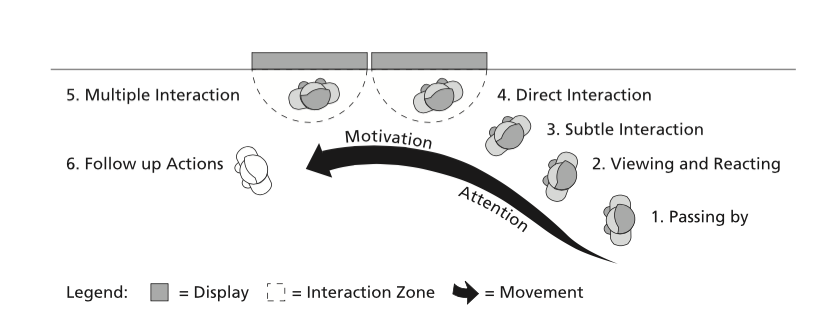
\includegraphics[width=120mm,height=70mm]{Figures/3/TheAudienceFunnel}
\caption{The Audience Funnel}
\label{fig:audience_funnel}
\end{figure}


\section{Attention}
Every moment we spend alone, with friends in the crowd, in the concert or party our attention keeps tracks of us and make us aware of the environment and we react for differently for different stimuli, so ``\emph{Attention is the process that, at a given moment, enhances some information and inhibits other information. The enhancement enables us to select some information for further processing, and the inhibition enables us to set some information aside.}''\cite{Attention}. Attention is influenced by two different processes (Top-Down \& Bottom-Up). Top-Down process happens when the user has prior awareness (goal) about where to put his/her attention toward and Bottom-Up process happens when the user has no prior awareness and suddenly by an external stimuli move or change attention toward or to something. People walking on pathway or walking in a store or waiting in bus station does not have any knowledge or awareness about an Interactive advertisements located there, nor the researches tend to speak about it for them, at this situation I believe that the attraction of attention should be a Bottom-Up process for the users to drag them to the screens.

The appearance of objects suddenly or moving objects on the screen or contrasting color can capture attention quicker. Yantis and Jonides (1984) demonstrated that the detection of a target in visual search was markedly enhanced when the target was presented as an abruptly\cite{capturingattention}. And the type of contrast change on an object influence priority in visual search, ``\emph{Both the sudden appearance of an object and sudden changes in existing object features influence priority in visual search.}''\cite{Luminance}

Elaine M. Huang, Anna Koster, and Jan Borchers have researched and discussed on ``\emph{When Does the Public Really Look at Public Displays ?}''\cite{WhenPublicDisplays}, in this paper they argued that glancing and attention at large displays is complex and is dependent on many factors like Brevity of glances, Positioning of displays, Content format and dynamics, Catching the eye, Display size, this paper provided some recommendations for each of the mentioned factors.


\section{Prototypes}
 
\begin{wrapfigure}[11]{r}{0.21\textheight} %this figure will be at the right
    \centering
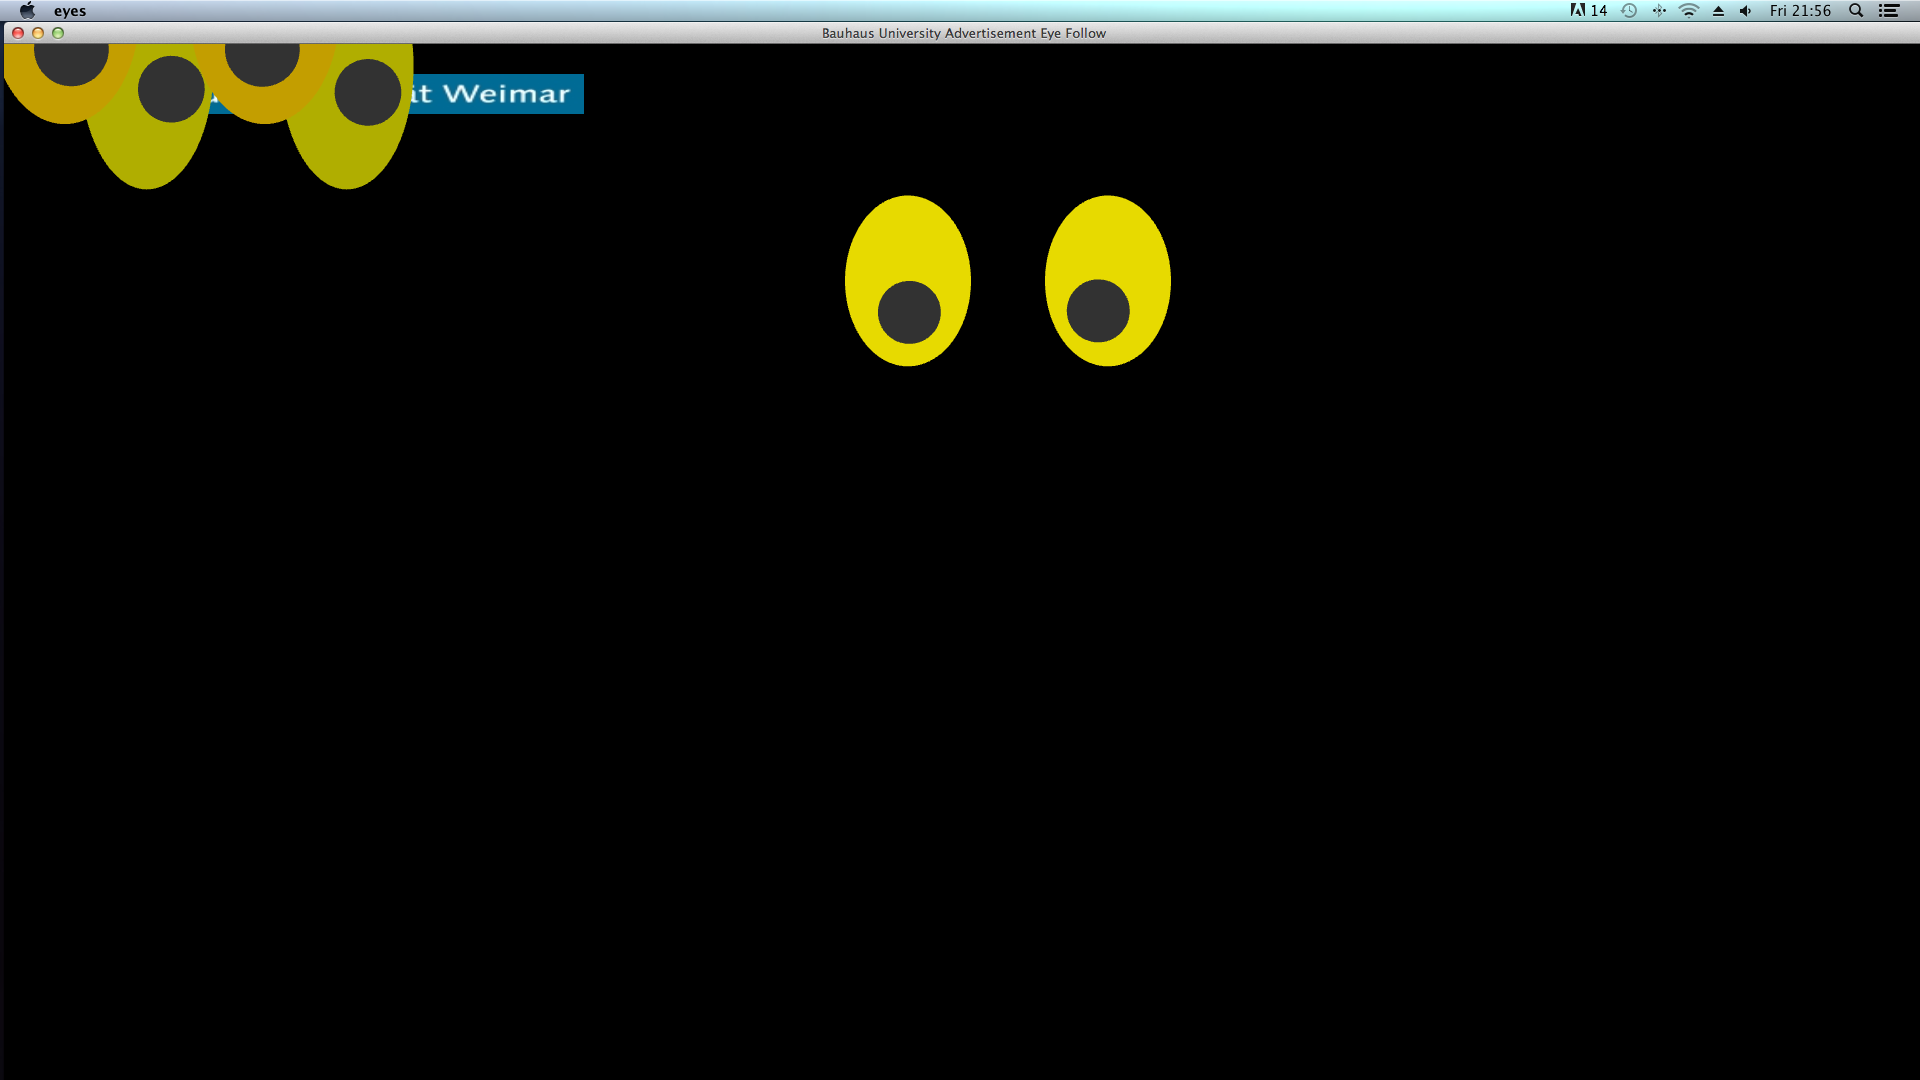
\includegraphics[width=50mm,height=40mm]{Figures/3/eyes}
\caption{following eyes}
\label{fig:eyes}
\end{wrapfigure} 
 
For the initial attention testing, three different types of eye-?catching techniques are made to observe which suites best for further research and which side of them should be improved and use them for the interactive advertisement. In this study the of the interactivity or the advertisement itself are not the core study, this study is only to see how many passer change their attention (glance) toward the screen. In the following examples the screen background color is set to black and is in full screen mode but with different contents. As you can see in this figure these eyes suddenly pop-up when a person pass by the screen and follows the person by moving its eyeball. The idea behind this is to check if people would react if something abruptly appear on the screen and starts to follow people, This example has very limited movement it is only constraint with limited eye space, but big object with high contrast.

\begin{wrapfigure}[10]{l}{0.21\textheight} %this figure will be at the right
    \centering
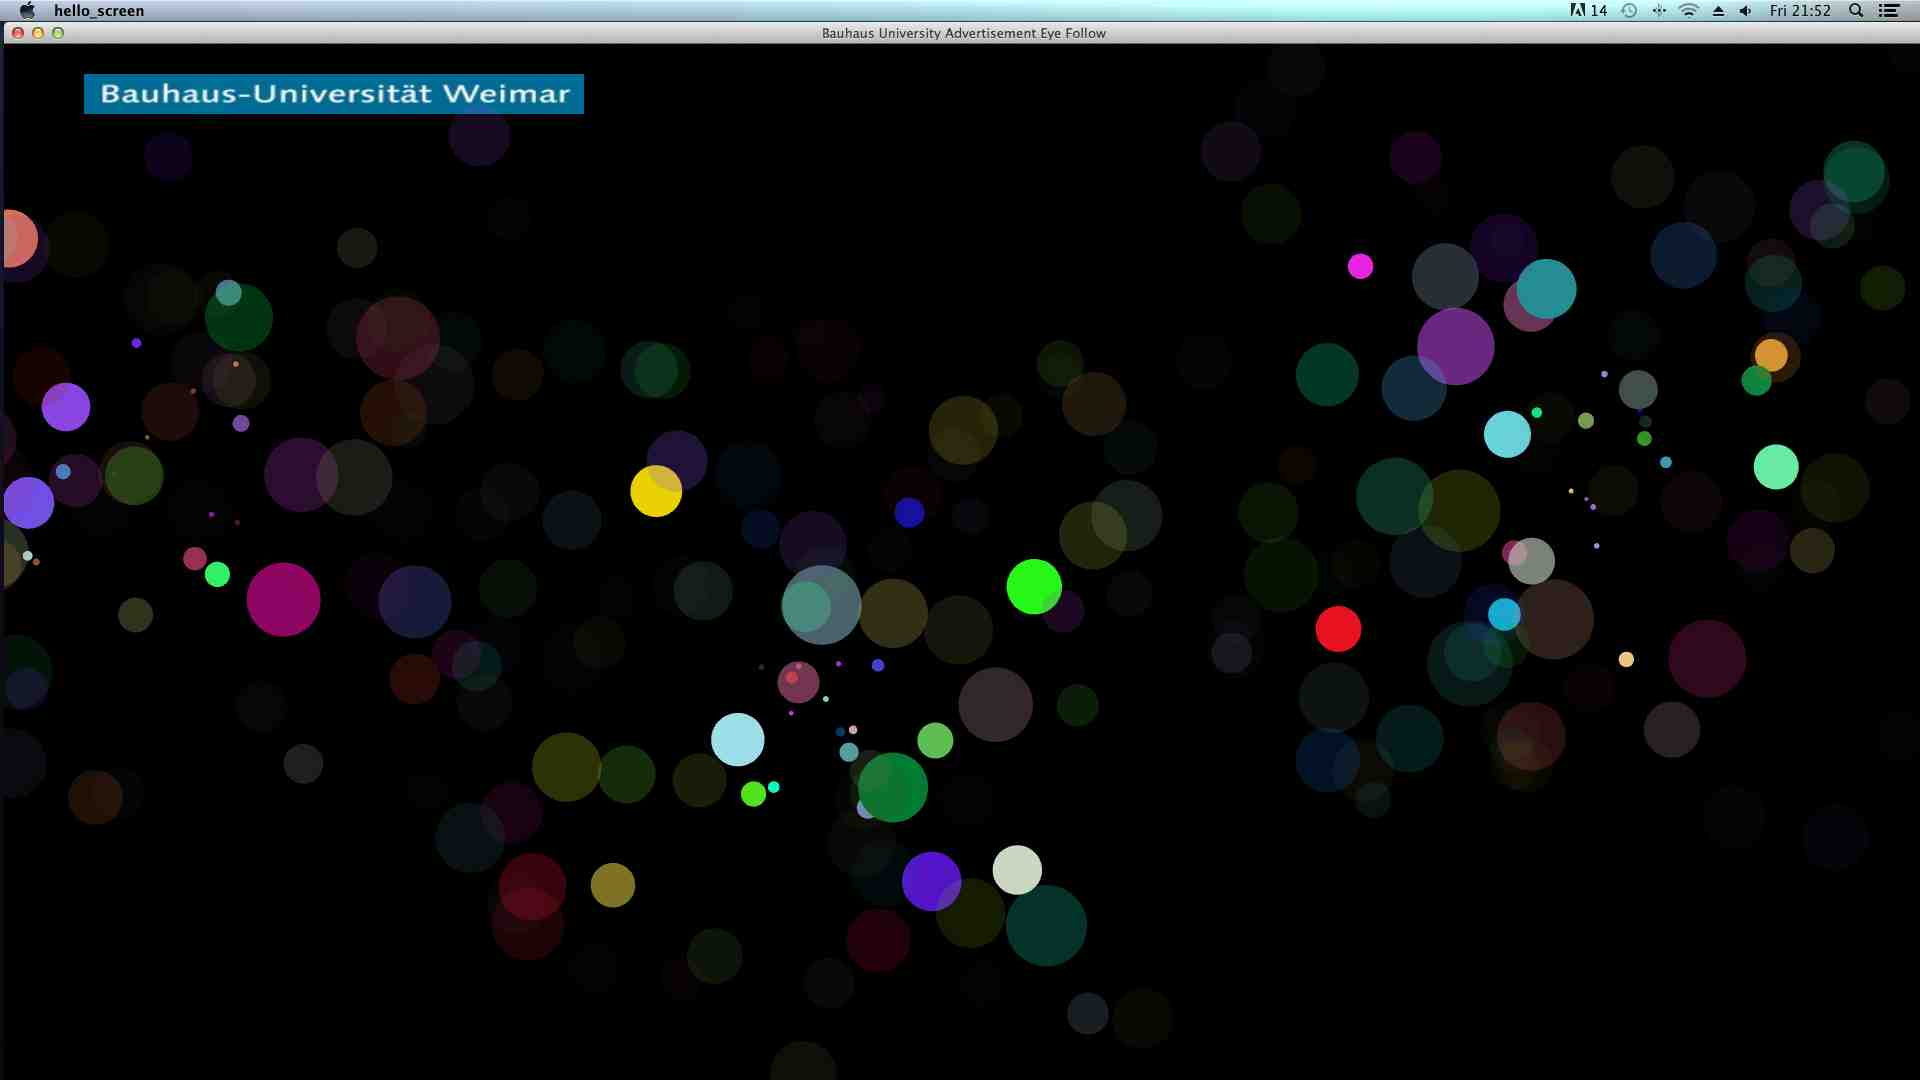
\includegraphics[width=50mm,height=40mm]{Figures/3/fireworks}
\caption{three Fireworks animation}
\label{fig:fireworks}
\end{wrapfigure}

\par
Another example in In figure 3, shows different colored and sized firework animation, The application will show a random firework for each person on the scene, there are three blocks of fireworks for three persons, the movement of the person changes the location of the firework. In this example there is more object movement and color changes with high contrast.

\newpage
\begin{wrapfigure}[11]{r}{0.21\textheight} %this figure will be at the right
    \centering
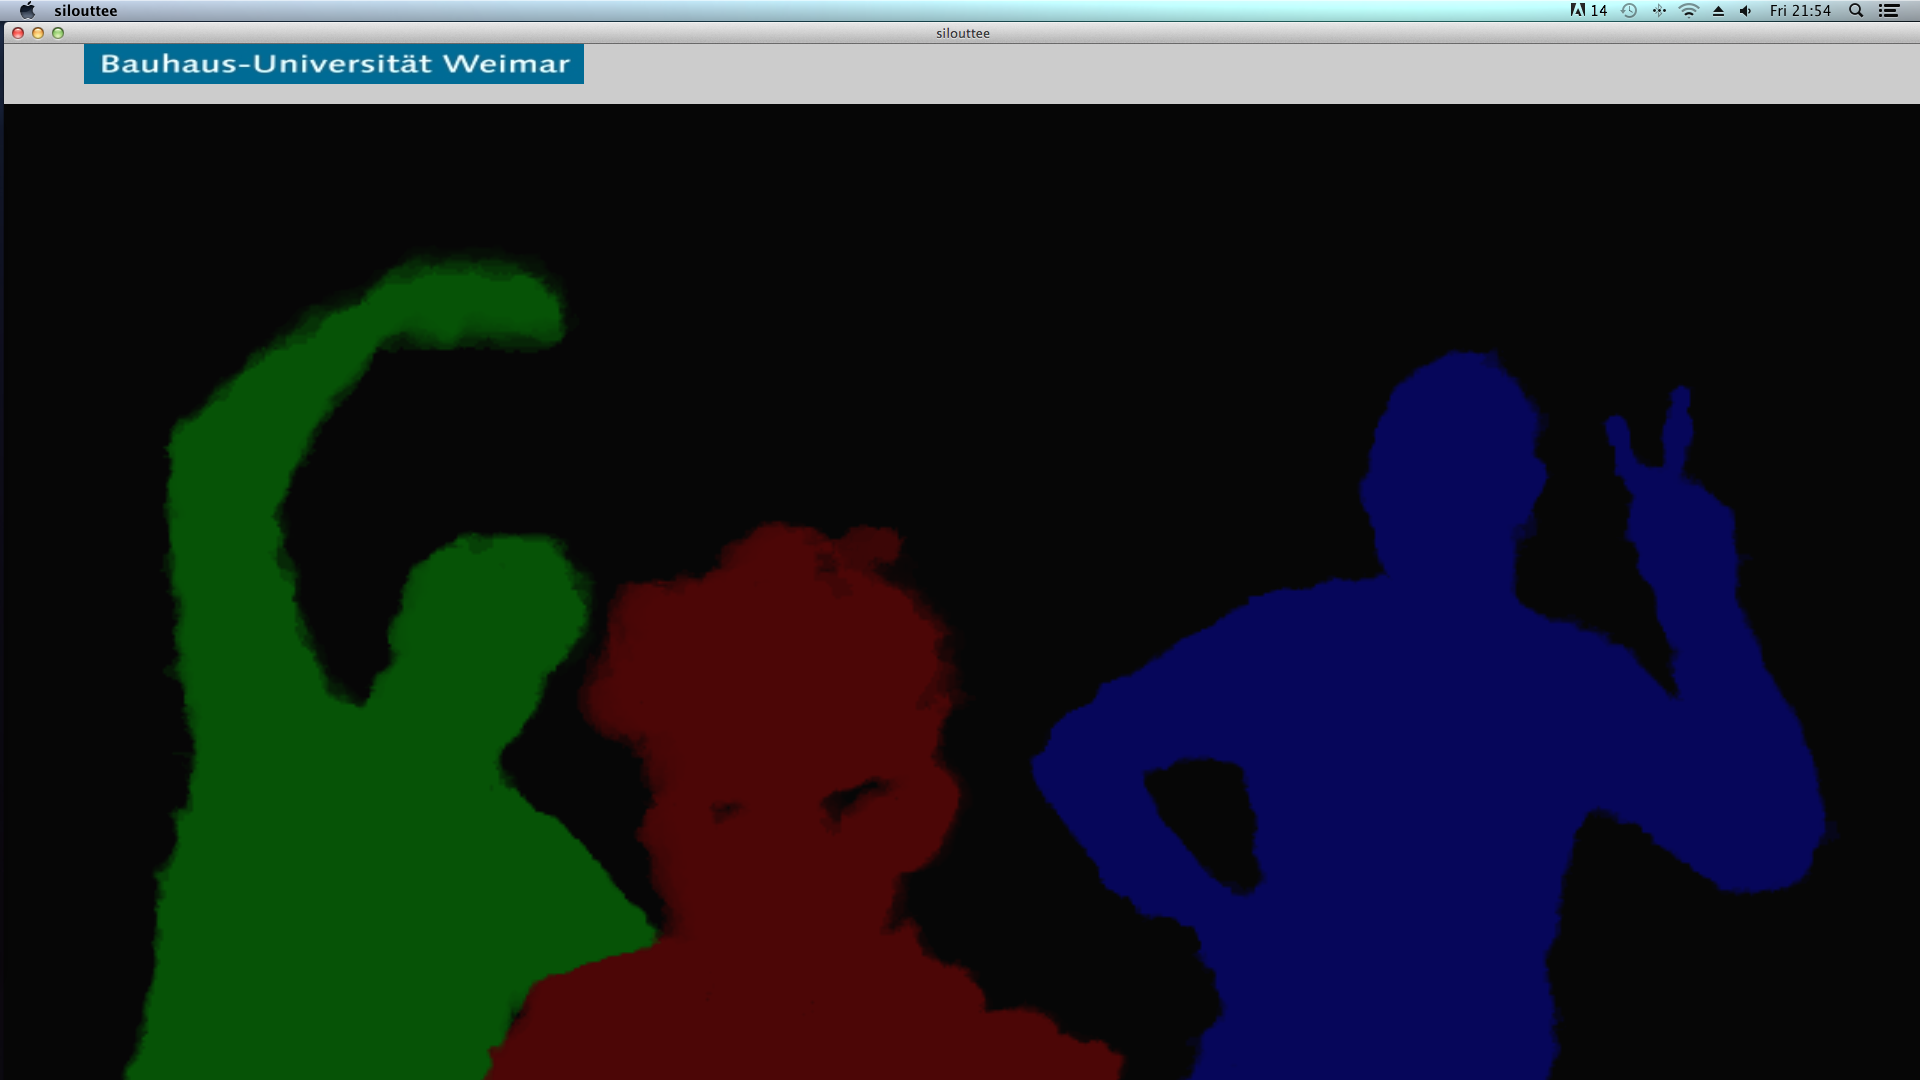
\includegraphics[width=50mm,height=40mm]{Figures/3/silhouttee}
\caption{three silhouette representation}
\label{fig:silhouttee}
\end{wrapfigure}


Jorg Müller \cite{LookingGlass} has investigated that how passers-by notice the?interactivity of the public display by showing different representations of body like Mirrored (1) user silhouettes, (2) avatar-like?representations and (3) real user Image. In that paper they concluded that mirroring user image is much more effective to attract?users and understand the interactivity of the display, but because of privacy policy and because of social attitude like may be someone does not like to be shown on the screen, i would show only  Mirrored silhouettes which is the augmented colored representation of people and see how much is the attraction toward the screen

\section{Study design}

The study will be a direct observation by me, which will be held in the university Mensa; the display will be installed near the stairs where already a small screen is there for advertisement. The first part of the study is the passive mode of the screen where traditional advertisement will be displayed for two days, For this study the immediate glance toward the screen will be investigated. The three mentioned examples will also be tested each two days and immediate glance and beside that other different effect like honeypot effect, the landing effect will also be investigated. The glance toward the screen is determined by the user head orientation, if the user turns his/her head up toward the screen, this will be considered as a glance. Honeypot effect \cite{EnticingPeople} describes the effect of people being attracted by persons already interacting with a device and Landing Effect \cite{LookingGlass}  is when people notice interactivity late and walks back toward the screen and does interaction.


\subsection{Hypothesis}


\begin{itemize}
\item \textbf{H1:} Interactive advertisements attract more people than traditional advertisement.
	
	\begin{enumerate}
		\item Dependent Variable: Number of people glance per total passers-by.
		\item Independent Variable : Interactive / traditional Advertisement.
	\end{enumerate}
		
\end{itemize}



\section{Data gathering}
Three different attraction attention methods and one traditional advertisement of Kasseturm were evaluated each for two hour period from 14:00--16:00 in individual days in Bauhaus University Mensa. Two methods (Observation and Interviews) were used for data gathering during the four day long period.

\subsection{Observation}
Observation was used to count the number of glances the passers-by make at the screen while pass from the front of the screen. A small pilot study was conducted for the observer to find an appropriate location in the Mensa setup to be able to count people and glances without being noticed by passers-by. The first day, which is a normal advertisement, does not require Kinect Camera, but in order to have same environment for all the days, I installed the camera on top of the monitor to look similar as the other interactive feature.

\begin{figure}[!htb]
    \centering
    \subfloat[]{{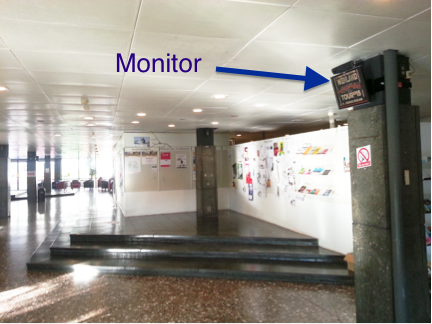
\includegraphics[width=6cm]{Figures/3/Kasseturm_monitor} }}%
    \hfill
    \subfloat[]{{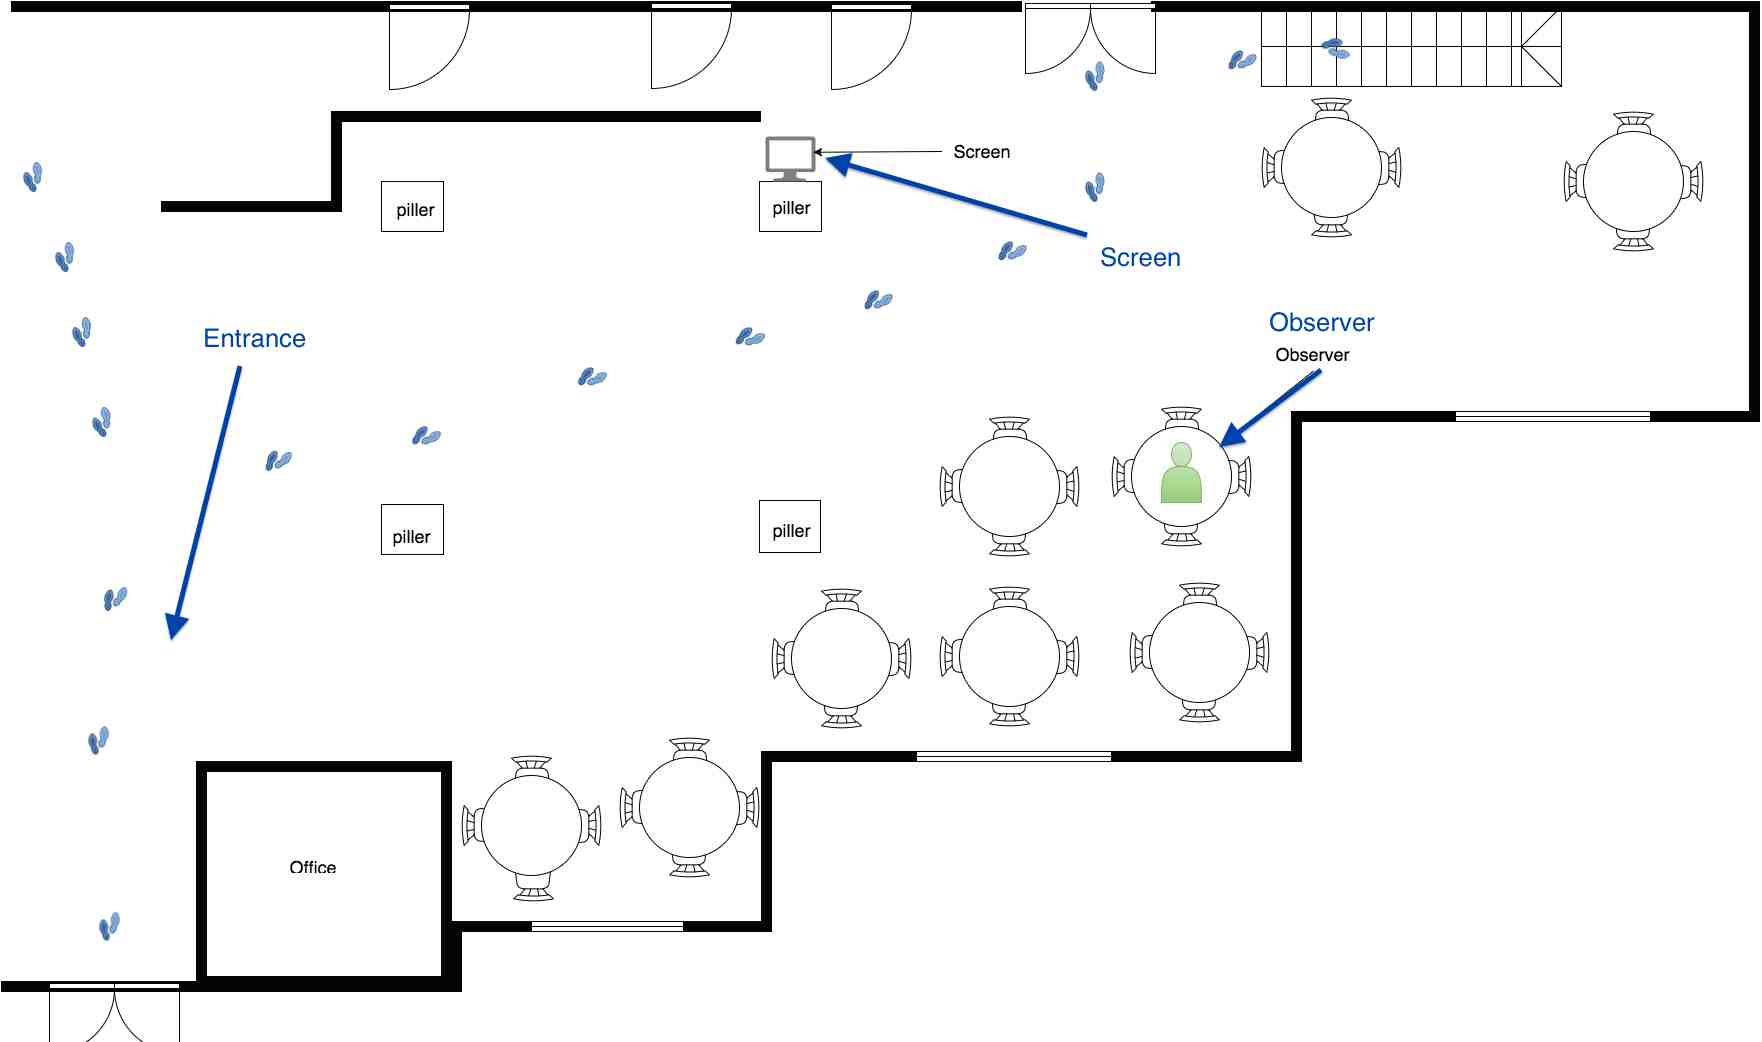
\includegraphics[width=6cm]{Figures/3/mensa_setup} }}%
    \caption{A: Mensa ground floor plan. B: Kasseturm Advertising monitor. }%
    \label{fig:observation_env}%
\end{figure}

As sheet was provided to the observer to note each 5 min time stamp for two hours, specific letters were defined to detect Male, Female, Unknown gender and at the same time who were in a group and individual and who glanced to the screen. 

%include the info sheet here
\newpage
As stated before that observer was given one small pilot study to detect a good location and be able to count and note in the sheet, beside that he was told to write notes if he observes something interesting during the period.

\begin{figure}[!htb]
    \centering
    \subfloat[]{{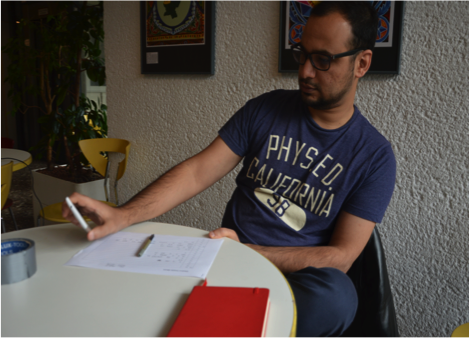
\includegraphics[width=6cm,height=4cm]{Figures/3/hamid} }}%
    \hfill
    \subfloat[]{{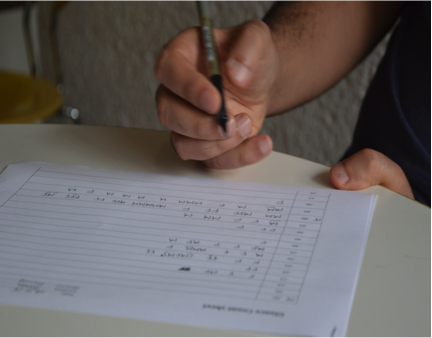
\includegraphics[width=6cm,height=4cm]{Figures/3/observer} }}%
    \caption{A: Hamid Sabri is getting prepared for observation. B: Observer is taking notes on the data sheet.. }%
    \label{fig:observation_env}%
\end{figure}




\subsection{Interviews}

During all four day of the observations, 16 interviews were taken from people inside Mensa to get general opinion about advertisement and people preferences what they like and what they avoid about advertisement. Responders were asked to sign the consent form because the interviews were tap recorded for later analyzing.  Each interview took around 6 minute in average. All interviews were transcribed separately for further data analyzing.

section{Findings}


\subsection{Observation findings}

Observational data for glance count and people passed by the screen were gathered and results to the bellow findings.

% table
\begin{table}[!htb]
\caption{Results of attraction attention methods}
\label{tab:treatments}
\centering
\begin{tabular}{l l l l }
\toprule
\tabhead{Method} & \tabhead{Glanced \%} & \tabhead{ingnored \%} & \tabhead{Total } \\
\midrule
Traditional & 9 \%7.6 & 109 \%92.3 & 118\\
Silhouette & 21 \%15.2 & 117 84.7 \%92.3 & 138\\
Following eye & 10 \%12.98 & 67 \%87 & 77\\
Firework & 6 \%10.1 & 53 \%89 & 59\\
\bottomrule\\
\end{tabular}
\end{table}

As can be seen a lot of from the table above Silhouette attention attraction technique received the highest number of glances 21 out of 138 compared to other techniques, Following eye technique was the second most attracted technique probably because of its contrasting color and funny.

\hilight{Attraction level has not changed between male and female}

So the decision would be to use silhouette technique for further advertisement application. 


\subsection{Interview Findings}

Interview transcripts were individually coded to generalize the responder?s opinions on the advertisements. I created two main sections from the interviews that what makes a Good Advertisement, and what makes a Bad Advertisement and related all responses to these sections a lot of codes were analyzed and grouped together to make sub sections and sub-sub-sections.

\subsubsection{Good Advertisement}
A lot of categories have been found after coding the interviews the chart in Appendix A, show all the categories and sub categories with the correspondent code from the interviews and even some codes were directly also placed as a category instance. The bellow list describes some of the important categories retrieved from the diagram.


\begin{enumerate}
\item \textbf{Content} \\
Interactive advertisements attract more people than traditional advertisement.
Responders like to have more Funny contents than any other restrict informational advertisement; ?just make it funny like make a joke or something but something in a very good one that is really difficult?, ?it should be very not very serious?, ?Yeah mostly I like funny things that the main concept is shown in different way like in funny things?, ?I like advertisement that are somehow have humor?. 	 \\

At the same time responders would like to see some useful, true, sensible facts and main idea of advertisement; ?an offer if it is clearly mentions that okay that you save this much or you get this or that, that is like a clear message?,  ?you have to focus on the main things that will happen in the event which will attract people will come.? \\

Furthermore contents of advertisement should be small and understandable; ?the advertisement should be clear too. ?, ?when you have too many numbers and too much to read then it is confusing?  ?Add some pictures based on the advertisement what do you want to show. ?, ?Not many text in advertisement?,? Have a good design, not too crowded with information?, ?Well defined subject, and shorter contents, because we don?t like reading long things usually no  body likes to read?.  \\

Another important thing was Context Based contents, the users liked to see things related to their surroundings; ?if I am standing near a shopping center it should tell me that what kind of shops are there and what I could buy from there.?  ?It should show movies of the actor I like?. \\
		
		
\item \textbf{Creativity} \\	
People like to see very new and creative things happening in advertisement; ?something that catches your attention in a way that you haven?t seen before?, ?like seeing something out of ordinary?. Introducing new ideas, artistic; ?as I am musician you know kind of creative person I like if it something special inside not it is just like for example if it is advertisement of milk ?, ?Which can be something un-expectable probably also ?, ?in general I would say yes as long it gets creative?


\item \textbf{Style} \\	
The style of advertisement plays key role in terms of color and size as stated by responders; ?may be should be more should be more colorful?, ?my eyes are attracted to so hard things unless there is something big enough things ?, ?Use the bright color. ?, ?You have to be clever in using colors okay because color mismatch does not attract the eyes?, ?when it is really just like an art like you have a picture you some impression or illusion?.

\item \textbf{Location} \\	
Responders like to see advertisement while they are on the way, they don?t get annoyed if advertisements comes on their way and some probably take a look to them too, but heavily they do not like advertisement while they are at home or watching program in TV or Internet, ?I think the street is better?

\item \textbf{Interactivity} \\	
Some liked to have some sort of interactivity to experience like playing games; ?it is good like if you have a game, it would better to have a preview of the game on the screen or just like something like even people could interact with it like get an experience of the game?, ?if the screen will also be interactive so you can interact with the with the something you are advertising.?

\item \textbf{Mean} \\
Different means were mentioned like larger screen, sound, banners for good influential advertisement.

\item \textbf{Motivation} \\
One of the responder pointed that the advertisement should motivate users in a natural way and should be from unbiased point of view; ?I prefer to buy in a natural way. The company should know who are using their product the power users who that have a lot of influence you know if you have good connections with the guitarists who have like actually like you know people listen to his opinion I think you have to reach out to the guitarist but once you know the guitarist is gaining something from that guitar maker then I don?t trust that company, It should be like completely unbiased, I think that is the kind of advertisement I listen to. ?. \\

Others suggest that advertisement must motivate for healthy diet and sport; ?if it reminds me to do stuff like do more sport or eat healthier or anything that has a good purpose?

\item \textbf{Other categories} \\
Many other categories were also extracted for a good advertisement like Goal of advertisement, Audience, Purpose and motivation, for more detail look at appendix A.
		
\end{enumerate}



\subsubsection{Bad Advertisement}
The bellow categories were derived from the interviews that make an advertisement feel or look bad, and we should not avoid using in advertisements.

\begin{enumerate}
\item \textbf{Style} \\
There exist different styles that advertisement makers follow but texts or photos are blinking; ?try not to use anything would be blinking okay because that is really annoying okay because even so if you are not looking at it is still effecting?. Using of mismatched colors in advertisement is certainly a bad idea; ?color mismatch does not attract the eyes?.

\item \textbf{Annoyance} \\
Most of the responders felt annoyed by almost all advertisements because they contain some sort of similar features like repetitions; ?it should not be like repeating itself over and over and over again?, ?I like advertisement apart from watching it again and again?, ?Hmm if I see the same advertisement again and again that is annoying. \\
? Other feature is destruction, which does not allow a person on focusing on something; ?Not just like something popping up in front of your face?, ?for example in middle of the serial or a movie that i am watching and an advertisement that is I don't like because it makes me destructed now I just can't focus on things for view minutes you have to leave what ever you were?

\item \textbf{Motivation} \\
Advertisement in general motivate people in their own way to attract customers, which people make not like it, for example sudden appearance of something in the screen or what users do not like to see but they are forced to see; ?usually you are forced to see them because you are watching something or doing something and suddenly it comes and it disturbs you?, ?it is trying to convince me of something only for to consume or buy and then I mean I don?t? want?

\item \textbf{Content} \\
Some advertisements exaggerate on their products or even say lie; ?it is like magnificent thing and nice pen okay and then it is just a pen, okay?, ?They are all lies?. Showing inappropriate content are heavily disliked; ?whenever I go and access the Internet okay? A lot of advertisement comes to my face and most of them are inappropriate. \\
Stuffs like that I don't like them at all?, ?for example some perfume ad which would the a woman in a very degrading position or for example mocking someone believe or something just to catch the attention that is probably to offend people that is what would annoy me a lot. ?. The use of ugly and old people is also not welcomed.

\item \textbf{Duration} \\
Long lasting advertisement are always boring and waste of time, most of the responders said that they would prefer short advertisements.

\item \textbf{Other categories} \\
Many other categories are also extracted from the interviews like location, Confusing advertisement, Controversial ads, amount of ads and types of ads that were not liked by responders. For more information see Appendix B

\end{enumerate}


\section{Discussions}

\section{Conclusion} 


